\chapter{Isogeny Based Cryptography}

In this chapter we will explain how isogenies of supersingular elliptic curves can be used for cryptography, and in particular for post-quantum secure protocols.

We will introduce the two main frameworks of isogeny crypto, namely SIDH and CSIDH, analyzing their inner workings, their hardness assumptions and their post-quantum security.

Some of the most useful resources on the subject are \cite{DeFeo_intro}, \url{https://defeo.lu/hdr} and \cite{Galbraith_SIproblems}.

\section{Diffie-Hellman key exchange}

One of the most important primitives in cryptography is the one of \emph{key exchange}, which allows two parties to obtain a shared secret between them while only communicating on public channels.

The main prototype of key exchanges is the one proposed by Diffie and Hellman in their seminal paper \cite{DH}, which marks the birth of the whole field of public key cryptography.

The DH protocol is very minimal, also in its setup: we fix a prime number $p$ and a generator $g$ of $\F_p^\ast$. Then the two parties Alice and Bob choose random values $a$ and $b$ respectively, and send each other the public values $A=g^a$ and $B=g^b$. The shared secret is then $g^{ab}$, which can be computed by Alice and Bob as $B^a$ and $A^b$, respectively.

This protocol is secure since solving the \emph{discrete logarithm problem} is hard, in the sense that there is no known algorithm that solves it in $O(\text{poly}(\log p))$ operations; for example, the generic baby-step giant-step algorithm has a running time of $O(\sqrt p)$, while the most optimized General Number Field Sieve has complexity $L_p[1/3,\sqrt[3]{64/9}]$\footnote{Recall that $L_n[\alpha, c]=\exp\left( (c+o(1))\log^\alpha(n)\log\log^{1-\alpha}(n) \right)$}.

Actually, since P vs NP is still an open problem, the whole field of cryptography works with assumptions and reductions: there is a small set of problems that are considered ``hard", and the proofs of security are simply reductions to one of those problems; more explicitly, most proofs use a format similar to ``suppose an adversary $\adv$ can break protocol $\pi$; then with the following steps $\adv$ can be used to solve an instance of the hard problem X".

We will not go into more details here (for example what \emph{break} means), since in the next chapter we will introduce the Universal Composability framework, which is one of the most general definitions of security for generic cryptographic protocols.

However we notice that for Diffie-Hellman there are at least two assumptions that can be made:
\begin{assumption}[DDH]
    The distributions $(g,g^a,g^b,g^{ab})$ and $(g,g^a,g^b,g^c)$ are computationally indistinguishable for random $a,b,c$, i.e. a polynomial-time adversary has a negligible probability of distinguishing them.
\end{assumption}
\begin{assumption}[CDH]
    Any polynomial-time adversary has a negligible probability of computing $g^{ab}$ from the knowledge of $g,g^a,g^b$.
\end{assumption}

For the naive version of the protocol, we notice that the decisional DH assumption can easily be broken with the use of Legendre symbols: if $g^a,g^b$ are both non residues, then $g^{ab}$ also isn't a square, while $g^c$ takes both square and non-square values.

Indeed one of the most useful abstractions of DH uses a group $G$ of prime order $q$, with a generator $g$. For finite field Diffie-Hellman this means taking $p=2q+1$ a Sophie-Germain prime, and $G={\F_p^\ast}^2$.

Another instantiation of Diffie-Hellman uses elliptic curves: we choose a curve $E$ over some finite field $\F_p$, we take a point $G\in E(\F_p)$ with prime order and use $G=\langle P\rangle$, the subgroup generated by $P$. In this case the operation $g^a$ becomes the scalar multiplication $[a]P$.

Those two protocols, called DH and ECDH, have been the core of public key cryptography, together with RSA, right from their discovery up until today. Indeed, any browser that visits a HTTPS website will probably check an RSA signature of the certificate, and then perform an ephemeral ECDH key exchange before encrypting all traffic with the newly obtained shared key.

However all instantiations of the DH protocol are now ``broken": in 1994 Shor published a polynomial-time quantum algorithm \cite{Shor94} that solves the discrete logarithm problem in any group. That day a race began between cryptographers trying to find \emph{post-quantum} alternatives, and many actors trying to actually build quantum computers able to perform discrete log computations on cryptographically sized input.

In the next sections we will thus introduce some new key exchange protocols which are based on isogenies of supersingular elliptic curves, whose problems are conjectured to be hard even for quantum computers.

In particular we will notice how CSIDH uses the action of an abelian group instead of group operations, while SIDH completely parts ways with groups and commutativity. A great introduction on these same topics can be found in \cite{Smith_DH}.


\section{History of isogeny-based cryptography}
With the discovery of Shor's order-finding algorithm for quantum computers in 1994 all public key cryptography known at the time was suddenly broken; even if not concretely, the presence of a polynomial quantum algorithm for what was believed a ``hard" problem was a shock to many computer scientists and cryptographers.

The roots of isogeny based cryptography lie shortly after Shor's algorithm: Jean-Marc Couveignes gave a talk in 1997 describing the first isogeny-based protocol, but it was published only ten years later in \cite{Couveignes}. It introduces the fundamental concept of \emph{Hard Homogeneous Spaces}, which is a generalization of Diffie-Hellman-like key exchanges using group \emph{actions} instead of the usual group operations.

Independently, Rostovtsev and Stolbunov proposed in \cite{Rostovtsev} a similar protocol using walks on isogeny graphs, or more precisely walks on the Cayley graph of the class group of some endomorphism ring.

Those papers introduced the main ideas of isogeny based cryptography, but were missing one fundamental detail: the use of \emph{supersingular} elliptic curves, both for faster isogeny evaluation and for improved security; those type of curves were indeed disregarded as ``bad" for cryptography, see \cite{Galbraith_sscurves} for example.

The true birth of isogeny crypto can be placed with the introduction of a hash function by Charles, Goren and Lauter in \cite{CGL}. They used the graph of supersingular elliptic curves over $\F_{p^2}$ with $\ell$-isogenies, proving its ``fast-mixing" properties.

In 2011 De Feo and Jao (and later Plut) introduced the \emph{Supersingular Isogeny Diffie-Hellman} protocol \cite{SIDH11}, which is probably the most famous isogeny protocol, since it's the only one that has been submitted to the NIST competition for post-quantum key exchanges algorithms, with the name of SIKE.

Another major breakthrough in isogeny crypto has been the implementation of the Couveignes protocol with supersingular curves, which led to the CSIDH protocol \cite{CSIDH}.

In the recent years there has been an exponential growth of isogeny based constructions for many different cryptographic primitives: mainly signatures (SeaSign \cite{SeaSign}, CSI-FiSh \cite{CSI-FiSh}, SQISign \cite{SQISign}), but also Verifiable Delay Functions \cite{DeFeo_VDF} and other MPC-friendly primitives like oblivious transfer, which will be our focus.

\section{Supersingular Isogeny Diffie-Hellman}
In this section we finally describe the SIDH protocol, introduced by Jao and De Feo in \cite{SIDH11}. Besides the actual paper, \cite{Costello_SIKE} is a tutorial for SIKE with all the computations for a toy example.

The high level view of this protocol can be understood with the following diagram:
\[\begin{tikzcd}
E \rar["\phi"] \dar["\psi"] & E/\langle P\rangle \dar\\
E/\langle Q\rangle \rar & E/\langle P, Q\rangle
\end{tikzcd}\]

where $E$ is a supersingular elliptic curve, the points $P$ and $Q$ are the secrets of Alice and Bob, the two quotients $E/\langle P\rangle$ and $E/\langle Q\rangle$ are the exchanged values and finally $E/\langle P, Q\rangle$ is the shared secret.

Moreover the two isogenies $\phi$ and $\psi$ are computed by a random walk in different degrees isogeny graphs.

The only thing that is not clear from this diagram is how to actually compute the right and bottom isogenies, without publishing $P$ or equivalently $\phi$.

Indeed, all the security of the protocol stands in the fact that it is hard for an attacker to recover the secret isogeny $\phi$, since the following problem is considered hard:
\begin{problem}
    Let $E,E'$ be two isogenous curves. Find an isogeny $\phi: E\to E'$.
\end{problem}

The trick to make the protocol work is to include in the public key some more information about $\phi$ than only its codomain. This is conjectured not to simplify much the isogeny finding problem, but still is a point that requires care, as we will see.

The protocol fixes a prime of the form $p=\ell_A^{e_A}\ell_B^{e_B}\cdot f\pm1$, where $\ell_A,\ell_B$ are small primes (usually $2$ and $3$) and $f$ is a small cofactor. Then it chooses a supersingular elliptic curve $E$ defined over $\F_q=\F_{p^2}$ with order $(\ell_A^{e_A}\ell_B^{e_B} f)^2$.

In this way $E[\ell_A^{e_A}]\subset E(\F_q)$, and since it's isomorphic to $\Zn{\ell_A^{e_A}}\times\Zn{\ell_A^{e_A}}$ it has $\ell_A^{e_A-1}(\ell_A+1)$ distinct cyclic subgroups of order $\ell_A^{e_A}$, each of which defines a different $\F_q$-isogeny. Thus the secret in this case is the kernel subgroup.

The other important step is to fix a basis $\{ P_A,Q_A \}$ of $E[\ell_A^{e_A}]$, and a basis $\{ P_B, Q_B \}$ of $E[\ell_B^{e_B}]$.

All these parameters are fixed by the protocol, and the actual key exchange is defined in figure \ref{prot_SIDH}.

\begin{figure}
    \myproc{Protocol SIDH}{
        \textbf{Alice} \> \> \textbf{Bob} \\
        a \sample \Zn{\ell_A^{e_A}} \> \> b \sample \Zn{\ell_B^{e_B}} \\
        A = P_A + [a]Q_A \> \> B = P_B + [b]Q_B \\
        \phi_A: E\to E_A=E/\langle A\rangle \> \> \phi_B: E\to E_B=E/\langle B\rangle\\
        \> \sendmessageright*{E_A, (\phi_A(P_B),\phi_A(Q_B))} \> \\
        \> \sendmessageleft*{E_B, (\phi_B(P_A),\phi_B(Q_A))} \> \\
        B' = \phi_B(P_A) + [a]\phi_B(Q_A) \> \> A' = \phi_A(P_B) + [b]\phi_A(Q_B) \\
        \phi'_A: E_B\to E_{BA}=E_B/\langle A'\rangle \> \> \phi'_B: E_A\to E_{AB}=E_A/\langle B'\rangle\\
        s=j(E_{BA}) \> \> s=j(E_{AB})
    }
    \caption{The SIDH protocol}
    \label{prot_SIDH}
\end{figure}

We can easily see that the protocol is correct, since both compositions $\phi'_A\circ\phi_B:E\to E_{BA}$ and $\phi'_B\circ\phi_A:E\to E_{AB}$ have the same kernel $\langle A,B\rangle$, thus are isomorphic and with the same $j$-invariant.

One of the most important details of this protocol isn't described in our sketched representation, but is the reason why we can actually perform the protocol as the honest users: the isogeny computation.

Indeed, blindly applying Vélu's formula for computing $\phi_A$ results in $O(\ell_A^{e_A})$ operations, which is roughly as much operations as an attacker needs to do in order to break the protocol.

Instead we use the fact that all our isogenies have \emph{smooth} degree, and thus can be computed as the composition of many small degree isogenies. In general, let $R$ be a point of order $\ell^e$ on the curve $E$; we will describe how to compute the isogeny $\phi:E\to E/\langle R\rangle$ and also how to compute the point $\phi(T)$ for any other $T$.

We will do that recursively, and start by setting $E_0=E$, $R_0=R$ and $T_0=T$. Then, for any $0\le i<e$ we compute (this time with Vélu's formulas) $$E_{i+1}=E_i/\langle [\ell^{e-i-1}R_i] \rangle$$ with the associated isogeny $\phi_i:E_i\to E_{i+1}$, and in particular $R_{i+1}=\phi_i(R_i)$ and $T_{i+1}=\phi_i(T_i)$. In the end, $E/\langle R \rangle=E_e$, and $\phi=\phi_{e-1}\circ\dots\circ\phi_0$.

With this algorithm, we can compute efficiently all the quotients, in time $O(e^2\ell)$. However, we can still do better with the implementation of the so called ``optimal isogeny strategies", which are one of the main improvements of the 2014 version of the paper \cite{SIDH14}.

One final implementation detail is that the curves are in Montgomery form, so that we can efficiently compute additions and isogenies with $x$ only arithmetic.

\subsection{From SIDH to SIKE}
The SIDH is a key exchange protocol, however we need some transformations to obtain provable cryptographic security. The algorithm submitted to NIST is a \emph{Key Encapsulation Method} (or KEM), which has been named SIKE. All the details on the SIKE protocol can be found in the official specification at \url{https://sike.org/files/SIDH-spec.pdf}.

First of all, they derive a public-key encryption scheme $\texttt{PKE}=(\kgen,\enc,\dec)$ in which the encryption/decryption part is given by a one-time pad with a key obtained through a random oracle from the shared $j$-invariant. In particular, if $m$ is the message and $c$ the ciphertext, the relation is $c=m\oplus H(j)$, where $H$ is some hash function.

Then this encryption scheme is turned into a $\texttt{KEM}=(\keygen, \encaps, \decaps)$ by means of the Hofheinz transform \cite{Hofheinz}, which adds some randomness in order not to have static public keys, which as we will see might be a problem for SIDH.

There are three proposed sets of fixed parameters (the prime $p$ and the starting elliptic curve $E_0$), each of which targets a different level of expected security; they are named \texttt{SIKEp434}, \texttt{SIKEp610} and \texttt{SIKEp751}, from the bit-length of $p$, and have expected quantum security of $128, 192, 256$ bits.

In terms of efficiency, the SIKE protocol has been heavily optimized in the last 10 years, in each level of abstraction: the use of Montgomery curves for efficient curve addition, improved Vélu's formulas, optimized $\F_{p^2}$ arithmetic even at the level of writing custom assembly for specific architectures.

For example, using the implementations on the official submission page \url{https://sike.org/},
we tested that the reference implementation uses around 900 million CPU cycles for the $\keygen$ algorithm of \texttt{SIKEp434}, while the optimized AMD64 implementation uses only 5 million cycles for the same operation. This means being able to run the three operations $\keygen$, $\encaps$, $\decaps$ in just around 10ms and thus might be a valid option for the TLS key exchange part.

Some more detailed benchmarks of the use of SIKE inside TLS can be found on \href{https://blog.cloudflare.com/the-tls-post-quantum-experiment/}{Cloudflare's} or \href{https://aws.amazon.com/it/blogs/security/round-2-hybrid-post-quantum-tls-benchmarks/}{Amazon's} blog posts.

\section{The SIDH hardness assumptions}
In this section we explore with more detail what are the problems and the concrete hardness assumptions for the SIDH protocol.

As we already saw, public keys in SIDH have ``more" information than what one usually expects. We now state precisely the computational problems on which the security of SIDH is based.

Let $p$ be a prime of the form $\ell_A^{e_A}\ell_B^{e_B}\cdot f\pm1$ and fix a supersingular curve $E_0/\F_{p^2}$ with basis $\{P_A,Q_A\}$ and $\{P_B,Q_B\}$ for $E_0[\ell_A^{e_A}]$ and $E_0[\ell_B^{e_B}]$ respectively, as in the SIDH protocol.

\begin{problem}[Decisional Supersingular Isogeny (DSSI) problem]
    Let $E_A$ be another supersingular curve over $\F_{p^2}$. Decide whether $E_A$ is $\ell_A^{e_A}$-isogenous to $E_0$ or not.
\end{problem}

\begin{problem}[Computational Supersingular Isogeny (CSSI) problem]
    Let $\phi_A:E_0\to E_A$ be an isogeny with kernel $\langle P_A+[a]Q_A \rangle$, where $a$ is sampled uniformly at random from $\Zn{\ell_A^{e_A}}$. Given $E_A, \phi_A(P_B),\phi_A(Q_B)$, compute a generator $R_A$ for the kernel of the isogeny $\phi_A$.
\end{problem}

The most specific isogeny problems for SIDH are then the following:

\begin{problem}[Supersingular Computational Diffie-Hellman (SSCDH) problem]
    Let $\phi_A:E_0\to E_A$ be the secret isogeny with kernel $\langle P_A+[a]Q_A \rangle$ and similarly $\phi_B:E_0\to E_B$, with secret $b$. Given the curves $E_A,E_B$ and the points $\phi_A(P_B),\phi_A(Q_B),\phi_B(P_A),\phi_B(Q_A)$ compute the $j$-invariant of the curve $E_0/\langle P_A+[a]Q_A,P_B+[b]Q_B \rangle$.
\end{problem}

\begin{problem}[Supersingular Decision Diffie-Hellman (SSDDH) problem]
    Let $\phi_A:E_0\to E_A$ and $\phi_B:E_0\to E_B$ be the isogenies of SSCDH. Distinguish the distributions
    \begin{itemize}
        \item $(E_A,E_B,\phi_A(P_B),\phi_A(Q_B),\phi_B(P_A),\phi_B(Q_A), E_{AB})$ with $$E_{AB}\cong E_0/\langle P_A+[a]Q_A,P_B+[b]Q_B \rangle$$
        \item $(E_A,E_B,\phi_A(P_B),\phi_A(Q_B),\phi_B(P_A),\phi_B(Q_A), E_C)$ with $$E_C\cong E_0/\langle P_A+[r]Q_A,P_B+[s]Q_B \rangle$$
        where $r,s$ are randomly sampled from $\Zn{\ell_A^{e_A}}$ and $\Zn{\ell_B^{e_B}}$ respectively.
    \end{itemize}
\end{problem}

Notice that we have the obvious reductions $\text{CSSI}\ge\text{SSCDH}\ge\text{SSDDH}$ and $\text{DSSI}\ge\text{SSDDH}$. However there are no known reductions in the other direction, but at the same time no algorithm that performs better on SSCDH compared to CSSI, for example.

Indeed, the public points $\phi_A(P_B),\phi_A(Q_B)$ allow any attacker to compute the action of $\phi_A$ on all $E_0[\ell_B^{e_B}]$, but there seems to be no reason why this information induces some behaviour on the seemingly unrelated $E_0[\ell_A^{e_A}]$.

Observe that the action of $\phi_A$ on $E_0[\ell_A^{e_A}]$ is all we need to solve CSSI, since we can write the equation $\phi_A(P_A)+[a]\phi_A(Q_A)=O_{E_A}$, where the points are known; we then get the secret $a$ from computing a discrete logarithm, which is easy on supersingular curves.

It is thus assumed that SSCDH and CSSI might be equivalent, but it seems very hard to prove it, and it might actually be false. The theorems regarding the security of SIKE are thus formulated in the following way:

\begin{theorem}
    In the random oracle model, the scheme \texttt{PKE} is $\indcpa$ if the problem SSCDH is hard.
\end{theorem}

\begin{theorem}
    If \texttt{PKE} is \indcpa, then the \texttt{KEM} scheme is \indcca.
\end{theorem}

The notions of encryption scheme, $\indcpa$ and random oracle model are the usual ones, and in this thesis are introduced and described in chapter \ref{chapter_UC}.

\subsection{How to break SIDH}
We now briefly discuss some attacks that greatly impacted the design choices and the bit security of SIKE.

One of the first algorithm for the generic isogeny-finding problem is by Delfs and Galbraith \cite{Delfs_Galbraith}, and computes an $\F_{p^2}$-isogeny from $E$ to $E'$ in $O(\sqrt p)$, by first finding walks into the $\F_p$-isogeny graph, and then finding an $\F_p$-isogeny in $O(\sqrt[4]p)$.

However, one of the features of SIDH is that we know the degrees of the isogenies; in this case we can use a simpler generic algorithm for collision finding, that is a meet-in-the-middle algorithm, or \emph{claw finding} algorithm: given the two curves $E$ and $E_A$, build the two trees on the $\ell_A$-isogeny graph starting from $E$ and $E_A$ with depth $e_A/2$; then search if there is a common leaf and join the two half-paths to compute the secret isogeny $\phi_A$.

This attack has a cost of about $O(\ell_A^{e_A/2})$ time and space; since we don't want imbalances in the security for Alice or Bob, the parameters are selected such that $\ell_A^{e_A}\simeq \ell_B^{e_B}\simeq \sqrt{p}$. Indeed, the parameters for the standardized protocol \texttt{SIKEp434} are $p=2^{216}3^{137}-1$.

In terms of quantum security, the claw finding algorithm can be optimized to run in $O(\sqrt[6]{p})$ instead of the classical $O(\sqrt[4]{p})$, as described in \cite{Tani_claw}.

There is also an optimization for parallelizing claw finding-like algorithm by van Oorschot and Wiener \cite{vOW}, which uses less memory but slightly more computation time. This is considered the main threat to SIKE, even if it's a completely generic algorithm.

Recently Microsoft has published two \href{https://www.microsoft.com/en-us/msrc/sike-cryptographic-challenge}{challenges} with reduced-size instances of SIKE, with bounties of \$5,000 and \$50,000, to improve the security analysis of SIKE. The smallest of the two has been broken by Udovenko and Vitto \cite{SIKE_challenge} this autumn; they did not use the vOW approach, but instead some clever optimizations of the claw finding algorithm, especially for the large memory required.


However, SIDH gives to the attacker also the action of the secret isogeny $\phi_A$ on the torsion subgroup $E[\ell_B^{e_B}]$. This is conjectured not to pose a serious threat, but there is an attack by Galbraith et al. \cite{Galbraith_SIKE} in the case that Alice runs many instances of SIDH with the same pair of keys.

We can describe two attack models, in terms of what is the output of Alice; in both cases the attack by Galbraith will recover the secret key $a\in\Zn{\ell_A^{e_A}}$ of Alice:
\begin{itemize}
    \item $O(E,R,S)=E/\langle R+[a]S\rangle$, i.e. Alice will complete her part of the key exchange and then will output the shared secret.
    \item $O(E,R,S,E')$ which outputs whether $j(E')=j(E/\langle R+[a]S\rangle)$; this model is more realistic, if for example Alice uses an authenticated encryption scheme with a key derived from the shared $j$-invariant, and returns an error when the authentication tag mismatches.
\end{itemize}

These attacks mean that SIDH can only be used as an interactive and ephemeral key exchange, and is the main reason behind the needed transformations in SIKE.

There are also other attacks exploiting the additional torsion point images in the public key \cite{SIDH_tp1, SIDH_tp2}; however, they target very particular parameter choices and some protocols derived from SIDH, but don't directly pose any threat to SIKE and its proposed standard parameters.

\section{Commutative SIDH}
In this section we describe the key exchange protocol CSIDH proposed by Castryck, Lange, Martindale, Panny and Renes \cite{CSIDH}. It is based on the ideas of Couveignes, but uses the supersingular component of the isogeny graph $G_\ell(\F_p)$ of curves defined over $\F_p$ for many different $\ell$. The use of supersingular curves is a speedup in walking the graph, since it makes the evaluation of the CM action much easier; actual implementations use key sizes of 64 bytes and the protocol is performed in about 80ms, which makes it actually usable in many applications.

The main point in favour of CSIDH is that it provides a \emph{non-interactive} key exchange protocol with static public keys, unlike SIDH which needs to be ephemeral. However, it suffers from a quantum subexponential attack; as the author themselves point out though, also RSA has a subexponential attack, but this didn't stop its widespread adoption.

More information and some implementations can be found at \url{https://csidh.isogeny.org/}.

\subsection{Hard Homogeneous Spaces}
The idea behind CSIDH was first proposed by Couveignes \cite{Couveignes} with his \emph{hard homogeneous spaces}, which are nothing but group actions where some problems are easy and some problems are hard.

\begin{definition}
    A hard homogeneous space consists of a finite abelian group $G$ acting freely and transitively on a set $X$.
    
    The following tasks are required to be easy (i.e. polynomial-time):
    \begin{enumerate}
        \item Computing group operations in $G$.
        \item Sampling from $G$ with almost uniform distribution.
        \item Deciding validity and equality of string representation of elements of $X$.
        \item Computing the action of a group element $g\in G$ on some $x\in X$.
    \end{enumerate}

    The following tasks are instead required to be hard (i.e. not polynomial-time):
    \begin{enumerate}
        \setcounter{enumi}{4}
        \item Vectorization: given $x,x'\in X$, find $g\in G$ such that $g\star x=x'$.
        \item Parallelization: given $x,x',y\in X$ with $g\star x=x'$, compute $y'\in X$ such that $g\star y=y'$.
    \end{enumerate}
\end{definition}

From any hard homogeneous space we can construct a natural Diffie-Hellman key exchange: Alice and Bob's private keys are random group elements $a,b\in G$, while their public keys are $a\star x_0$ and $b\star x_0$ for some fixed element $x_0\in X$; the shared secret is then $a\star(b\star x_0)=b\star(a\star x_0)$.

Notice how traditional DH on a cyclic group $C$ is an instance of this, with $X$ the set of generators of $C$, and $G$ the multiplicative group $(\Zn{\# C})^\ast$ acting by exponentiation.

In Couveignes' idea and in CSIDH the hard homogeneous space is given by the CM action on elliptic curves over $\F_p$.

Recall that given an elliptic curve $E/\F_p$ its endomorphism ring (defined over $\F_p$) $\End_p(E)$ is an order $\Oc$ in a quadratic imaginary field $K$. Denoting by $Ell_p(\Oc)$ the set of curves having $\Oc$ has their $\F_p$-endomorphism ring, we know there is the free and transitive action of $Cl(\Oc)$:
\begin{align*}
    Cl(\Oc)\times Ell_p(\Oc) & \to  Ell_p(\Oc)\\
    \mathfrak{a}\cdot E & \mapsto  E/\mathfrak{a}
\end{align*}

Notice that for cryptographically sized parameters we can't compute the structure of $Cl(\Oc)$, as $\# Cl(\Oc)\approx \sqrt{|\Delta|}$, where $\Delta$ is the discriminant of $\Oc$.

However, we can consider the map $\varphi:\Z^n\to Cl(\Oc)$ given by
$$(x_1,\dots,x_n)\mapsto \prod_{i=1}^n[\mathfrak{l}_i]^{x_i},$$
where the $\mathfrak{l}_i$ are the ideals corresponding to a subset of the Elkies primes (usually the ones of size up to some bound $B$).

Since the action of the $\mathfrak{l}_i$ is more easily computable, this will be our representation of the class group. Indeed, in the CSIDH protocol private keys will be tuples of integers.

This idea of Couveignes, as well as the approach by De Feo, Kieffer and Smith \cite{DeFeo_CSIDH}, are still inefficient, since usually there are very few small Elkies primes, while the computation of the isogeny corresponding to $\mathfrak{l}_i$ takes linear time in its norm.

\subsection{The CSIDH protocol}
The main idea of CSIDH is to pick a prime of the form $p=4\ell_1\dots\ell_n-1$, with $\ell_i$ small primes. Moreover they fix $E_0: y^2=x^3+x$, which is supersingular since $p\equiv3\pmod 4$; this curve has $\End_p(E_0)\cong\Z[\pi]$ which is an order inside $\Q(\sqrt{-p})$, of conductor $2$.

The Elkies primes are those which split as $\ell\Oc=\mathfrak{l}\cdot\bar{\mathfrak{l}}$, i.e. those that satisfy $\left( \frac{-p}{\ell} \right)=1$; since $p\equiv-1\pmod{\ell_i}$, we have that all the selected primes $\ell_i$ are Elkies. Moreover, since the characteristic polynomial of the Frobenius is $\pi^2+p=0$, when reduced modulo $\ell_i$ it becomes $\pi^2-1\equiv0\pmod{\ell_i}$; this means that $\ell$ splits as the product of $\mathfrak{l}_i=(\ell_i, \pi-1)$ and $\bar{\mathfrak{l}_i}=(\ell_i, \pi+1)$.

In this setting we use theorem \ref{CSIDH_cycle} to get that the horizontal level of $E_0$ in $G_{\ell_i}(\F_p)$ is a cycle, which can be traversed in both ways with $[\mathfrak{l}_i]$ and $[\bar{\mathfrak{l}_i}]=[\mathfrak{l}_i]^{-1}$. For CSIDH we are using the floor of this volcano, while there is a variant named \emph{CSURF} that uses the elliptic curves on the surface, which has been introduced by Castryck and Decru \cite{CSURF} and is slightly more efficient.

\begin{figure}
    \centering
    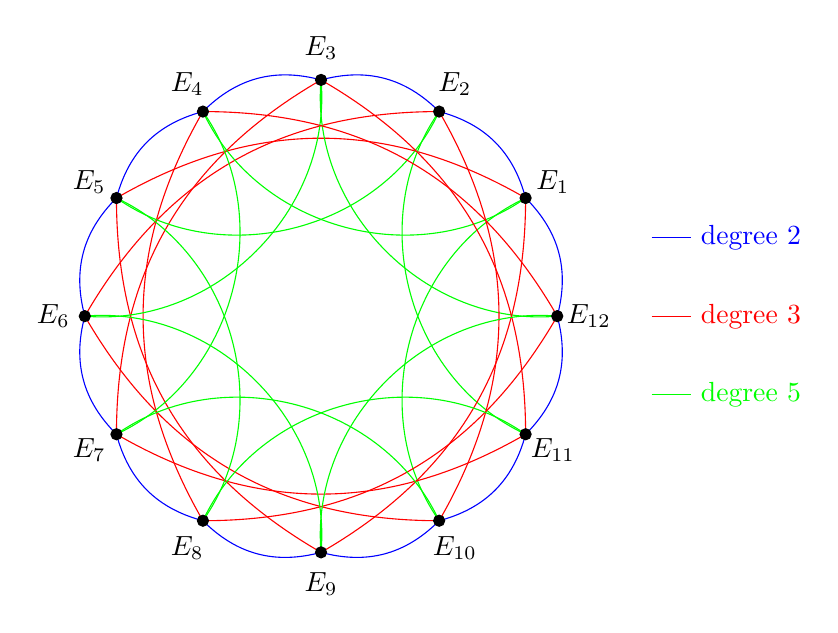
\begin{tikzpicture}
    \begin{scope}
    \def\crater{12}
    \def\jumpa{-8}
    \def\jumpb{9}
    \def\diam{3cm}
    
    \foreach \i in {1,...,\crater} {
        {\draw[blue] (360/\crater*\i : \diam) to[bend right] (360/\crater*\i+360/\crater : \diam);}
        {\draw[red] (360/\crater*\i : \diam) to[bend right] (360/\crater*\i+\jumpa*360/\crater : \diam);}
        {\draw[green] (360/\crater*\i : \diam) to[bend right=50] (360/\crater*\i+\jumpb*360/\crater : \diam);}
    }
    \foreach \i in {1,...,\crater} {
        \draw[fill] (360/\crater*\i: \diam) circle (2pt) +(360/\crater*\i: 0.4) node{$E_{\i}$};
    }
    \end{scope}
    \begin{scope}[xshift=4.2cm,yshift=1cm]
    
    {\draw[blue] (0,0) -- (0.5,0)
        (0.5,0) node[anchor=west] {degree $2$};}
    {\draw[red] (0,-1) -- (0.5,-1) (0.5,-1)
        node[anchor=west] {degree $3$};}
    {\draw[green]
        (0,-2) -- (0.5,-2) (0.5,-2) node[anchor=west] {degree $5$};}
    
    \end{scope}
    \end{tikzpicture}
    \caption{An abstract example of a CSIDH graph; picture by De Feo}
    \label{picture_CSIDH}
\end{figure}

Putting together the graphs for the different $\ell_i$, we get a picture similar to Figure \ref{picture_CSIDH}, which can be called a CM graph, or in this case a CSIDH graph.

The very peculiar choice of the prime $p$ implies that the evaluation of the action $\mathfrak{l}_i\cdot E$ is very easy: the kernel of the corresponding isogeny $E[\mathfrak{l}_i]$ is the intersection of $\ker[\ell_i]$ and $\ker(\pi-1)$, which is the $\F_p$-rational $\ell_i$-torsion subgroup. By computing it and using Vélu's formulas we can compute the isogeny $\varphi_{\mathfrak{l}_i}$.

For computing $\mathfrak{l}_i^{-1}\cdot E$ we can either compute the $\F_{p^2}$-rational $\ell_i$-torsion, or we can use the fact that $(\mathfrak{a}\cdot E)^t\cong\mathfrak{a}^{-1}\cdot E^t$, where $E^t$ is the quadratic twist of $E$. For more details on evaluating the class group action, we refer to \cite[section 8]{CSIDH}.

Another key aspect of CSIDH is that it uses curves in Montgomery form, because of the following proposition.
\begin{proposition}
    Let $p\ge5$ be a prime with $p\equiv3\pmod8$, and let $E/\F_p$ be a supersingular elliptic curve. Then $\End_p(E)=\Z[\pi]$ if and only if there exists $A\in\F_p$ such that $E$ is $\F_p$-isomorphic to the curve $E_A:y^2=x^3+Ax^2+x$. Moreover, such $A$ is unique.
\end{proposition}

This means that it is sufficient to use the $A$ coefficient as the public key, instead of a $j$-invariant and then having to check that it has the correct endomorphism ring. The only check needed is that $A\not\in\{\pm2\}$ (otherwise $E_A$ isn't even smooth), and that $E_A$ is supersingular.

Furthermore, it's very easy to see that in our setting (in particular given $p\equiv3\pmod 4$), the twist of $E_A$ is simply $E_A^t\cong E_{-A}$.

Finally, the CSIDH protocol is described in Figure \ref{prot_CSIDH}, where all above observation apply. In particular, private keys are tuple of integer exponents $(e_1,\dots,e_n)$, which correspond to the ideal $\prod [\mathfrak{l}_i]^{e_i}$; every $e_i$ is uniformly sampled from $\{ -m,\dots,m \}$, where $m$ is a fixed protocol parameter and must balance efficiency and security. The authors argue that if $2m+1\ge\sqrt[n]{\# Cl(\Oc)}$ the ideal sampled in this way is sufficiently close to the uniform distribution.

One example set of parameters is given by the proposed \texttt{CSIDH-512}, where $p=4\cdot\ell_1\cdots\ell_{74}-1$, with $\ell_1,\dots,\ell_{73}$ the first $73$ odd prime numbers, while $\ell_{74}=587$ (the smallest prime to make also $p$ be a prime); moreover the private exponents are chosen in $\{ -5,\dots,5 \}$.

\begin{figure}
    \begin{framed}
        \textbf{Setup}: A prime $p=4\ell_1\cdots\ell_n-1$, where $\ell_i$ are small distinct odd primes; $E_0:y^2=x^3+x$ is the base supersingular elliptic curve with $\Oc:=\End_p(E_0)=\Z[\pi]$. Fix also a parameter $m$.
        
        \textbf{Key generation}: Sample a tuple of integers $(e_1,\dots,e_n)$ from $\{ -m,\dots,m \}^n$. This tuple corresponds to the ideal $[\mathfrak{a}] = \prod [\mathfrak{l}_i]^{e_i}$ of $Cl(\Oc)$, where $\mathfrak{l}_i=(\ell_i, \pi-1)$. The public key is the $A$ coefficient of the curve $[\mathfrak{a}]E_0:y^2=x^3+Ax^2+x$ in Montgomery form.
        
        \textbf{Key exchange}: Suppose Alice and Bob have key pairs $([\mathfrak{a}], A)$ and $([\mathfrak{b}], B)$. When receiving $B$ from Bob, Alice checks the validity of this public key and then computes the curve $[\mathfrak{a}]E_B$. Bob does the same and computes $[\mathfrak{b}]E_A$. The shared secret is the Montgomery coefficient $S$ of the curve $[\mathfrak{a}][\mathfrak{b}]E_0=[\mathfrak{b}][\mathfrak{a}]E_0$ written as $y^2=x^3+Sx^2+x$.
    \end{framed}
    \caption{The CSIDH protocol}
    \label{prot_CSIDH}
\end{figure}


\section{CSIDH assumptions}
The main hardness assumptions for CSIDH security are the vectorization and the parallelization tasks of the hard homogeneous space of which CSIDH is an instance. In particular, we will analyze the following problem.

\begin{problem}[CSIDH problem]\label{problem_csidh}
    Given two supersingular curves $E,E'$ both defined over $\F_p$ and with the same $\F_p$-endomorphism ring $\Oc$, \emph{find} an ideal $\mathfrak{a}$ of $\Oc$ such that $[\mathfrak{a}]E=E'$. The ideal must be given in such a way that its action on the curve can be computed efficiently.
\end{problem}

We could also define the problems for parallelization and more, but we will do so when needed. Here we only notice that the analog of the DH decision problem has been ``broken" in \cite{breaking_DDH}, in a similar way in which the Legendre symbol ``breaks" DDH.

The most basic security analysis of CSIDH can be made by reusing the meet-in-the-middle approaches against SIDH. This results in a $O(\sqrt[4]{p})$ classical attack and a $O(\sqrt[6]{p})$ quantum attack, exactly as in SIDH.

However, the use of a commutative group reduces the quantum security of CSIDH, due to a family of subexponential quantum algorithms for solving the \emph{hidden shift problem} by Kuperberg \cite{Kuperberg2005} and Regev \cite{Regev_hshp}.
\begin{definition}
    Let $f_0,f_1:G\to X$ be two injective functions from a group $G$ to a set $X$. Suppose that there exists an element $s\in G$ such that $f_0(g)=f_1(gs)$ for any $g\in G$; this element $s$ is called a \emph{hidden shift} for $f_0,f_1$. The \emph{hidden shift problem} is to find $s$, given access to $f_0,f_1$.
\end{definition}
As noted in \cite{Childs_hshsp}, Kuperberg's algorithm can be used to solve the CM problem as follows: let $E_0,E_1$ be two curves with CM by $\Oc_K$ and define $f_0,f_1:Cl(\Oc_K)\to Ell_p(\Oc_K)$ by $f_i([\mathfrak{a}]) = [\mathfrak{a}]E_i$; this gives rise to an hidden shift that is precisely an horizontal isogeny between $E_0$ and $E_1$.

Since running time of those quantum algorithm is about $O(2^{\sqrt{\# G}})$, this means that for $n$-bit quantum security we need $\log p$ to be about $O(n^2)$.
    
The precise quantum cost in time and space for breaking CSIDH is still being debated; see \cite{CSIDH_Peikert}, \cite{CSIDH_BS}, \cite{CSIDH_qiso} and the most recent version of the CSIDH paper.

The authors argue that \texttt{CSIDH-512} might not fall too short of the $128$ classical bits of security, especially since evaluating isogenies adds much complexity to the quantum circuits.

\section{Equivalence of isogeny problems}
$\ell$-IsogenyPath vs. EndRing \cite{Weso_EndRing}.

Deuring correspondence computational aspects and KLPT.

\cite{Weso_CSIDH}
